
\documentclass{article}

\usepackage{fullpage,latexsym,picinpar,amsmath,amsfonts,graphicx}



\setlength{\evensidemargin}{0.1in}
\setlength{\oddsidemargin}{0.1in}
\setlength{\textwidth}{6.6in}
\setlength{\topmargin}{0.0in}
\setlength{\textheight}{8.7in}
\setlength{\headheight}{0in}
\setlength{\headsep}{0in}
\setlength{\topsep}{0in}
\setlength{\itemsep}{0in}
\renewcommand{\baselinestretch}{1.1}
\parskip=0.080in

\newcommand{\parend}[1]{{\left( #1  \right) }}
\newcommand{\spparend}[1]{{\left(\, #1  \,\right) }}
\newcommand{\angled}[1]{{\left\langle #1  \right\rangle }}
\newcommand{\brackd}[1]{{\left[ #1  \right] }}
\newcommand{\spbrackd}[1]{{\left[\, #1  \,\right] }}
\newcommand{\braced}[1]{{\left\{ #1  \right\} }}
\newcommand{\leftbraced}[1]{{\left\{ #1  \right. }}
\newcommand{\floor}[1]{{\left\lfloor #1\right\rfloor}}
\newcommand{\ceiling}[1]{{\left\lceil #1\right\rceil}}
\newcommand{\barred}[1]{{\left|#1\right|}}
\newcommand{\doublebarred}[1]{{\left|\left|#1\right|\right|}}
\newcommand{\spaced}[1]{{\, #1\, }}
\newcommand{\suchthat}{{\spaced{|}}}
\newcommand{\numof}{{\sharp}}

\newcommand{\half}{{\textstyle\frac{1}{2}}}
\newcommand{\elevenhalves}{{\textstyle\frac{11}{2}}}
\newcommand{\onethird}{{\textstyle\frac{1}{3}}}
\newcommand{\sixteenthirds}{{\textstyle\frac{16}{3}}}
\newcommand{\twentytwothirds}{{\textstyle\frac{22}{3}}}
\newcommand{\onefifth}{{\textstyle\frac{1}{5}}}
\newcommand{\threefifths}{{\textstyle\frac{3}{5}}}
\newcommand{\sixfifths}{{\textstyle\frac{6}{5}}}
\newcommand{\eightfifths}{{\textstyle\frac{8}{5}}}
\newcommand{\sixteenfifths}{{\textstyle\frac{16}{5}}}
\newcommand{\eightteenfifths}{{\textstyle\frac{18}{5}}}
\newcommand{\threetenths}{{\textstyle\frac{3}{10}}}
\newcommand{\twentysixfifteenths}{{\textstyle\frac{26}{15}}}
\newcommand{\fisefiftieths}{{\textstyle\frac{57}{50}}}
\newcommand{\ftwotfifths}{{\textstyle\frac{42}{25}}}
\newcommand{\fotwontwfifths}{{\textstyle\frac{42}{125}}}
\newcommand{\eithontwfifths}{{\textstyle\frac{83}{125}}}

\newcommand{\veps}{{\varepsilon}}
\newcommand{\Sigmastar}{{\Sigma^\ast}}

\newcounter{exnum}[section]
\newenvironment{problem}{{\vskip 0.1in
   \noindent \bf Problem\addtocounter{exnum}{1}~\arabic{exnum}.}}{\vskip 0.1in}

\newtheorem{theorem}{Theorem}
\newtheorem{definition}{Definition}
\newtheorem{corollary}{Corollary}
\newtheorem{lemma}{Lemma}
\newtheorem{fact}{Fact}
\newtheorem{claim}{Claim}

\newenvironment{proof}{{\it Proof:\/}}{$\Box$\vskip 0.1in}

\newcommand{\emparagraph}[1]{{\smallskip\noindent{\em #1\/}}}

\newcommand{\assign}{{\,\gets\,}}


%\newcommand{\hwduedate}{{}}

\begin{document}

\centerline{\large \bf CS/MATH111 ASSIGNMENT 5}
%\centerline{due {\hwduedate}}


\vskip 0.25in

%%%%%%%%%%%%%%%%

\begin{problem}
Determine whether the two graphs below are planar or not.
To show planarity, give a planar embedding.
To show that a graph is not planar, use Kuratowski's theorem.

\bigskip

\begin{center}
{\large Graph $G$:\ }
\begin{minipage}{2.1in}
        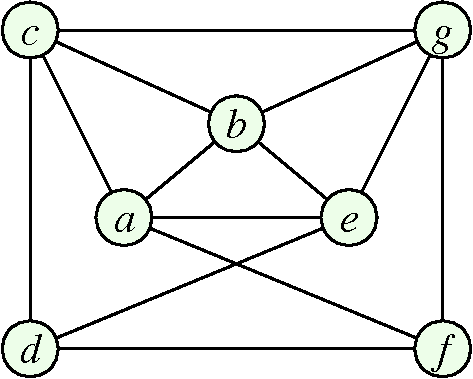
\includegraphics[width=1.75in]{planar_graphG_hw5.pdf}
\end{minipage}
\hfill
{\large Graph $H$:\ }
\begin{minipage}{2.4in}
        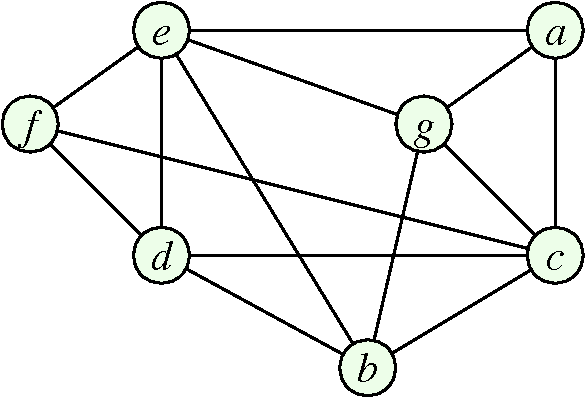
\includegraphics[width=2in]{planar_graphH_hw5.pdf}
\end{minipage}
\end{center}

\bigskip

\begin{center}
{\large Graph $G$:\ }
\begin{minipage}{2.1in}
		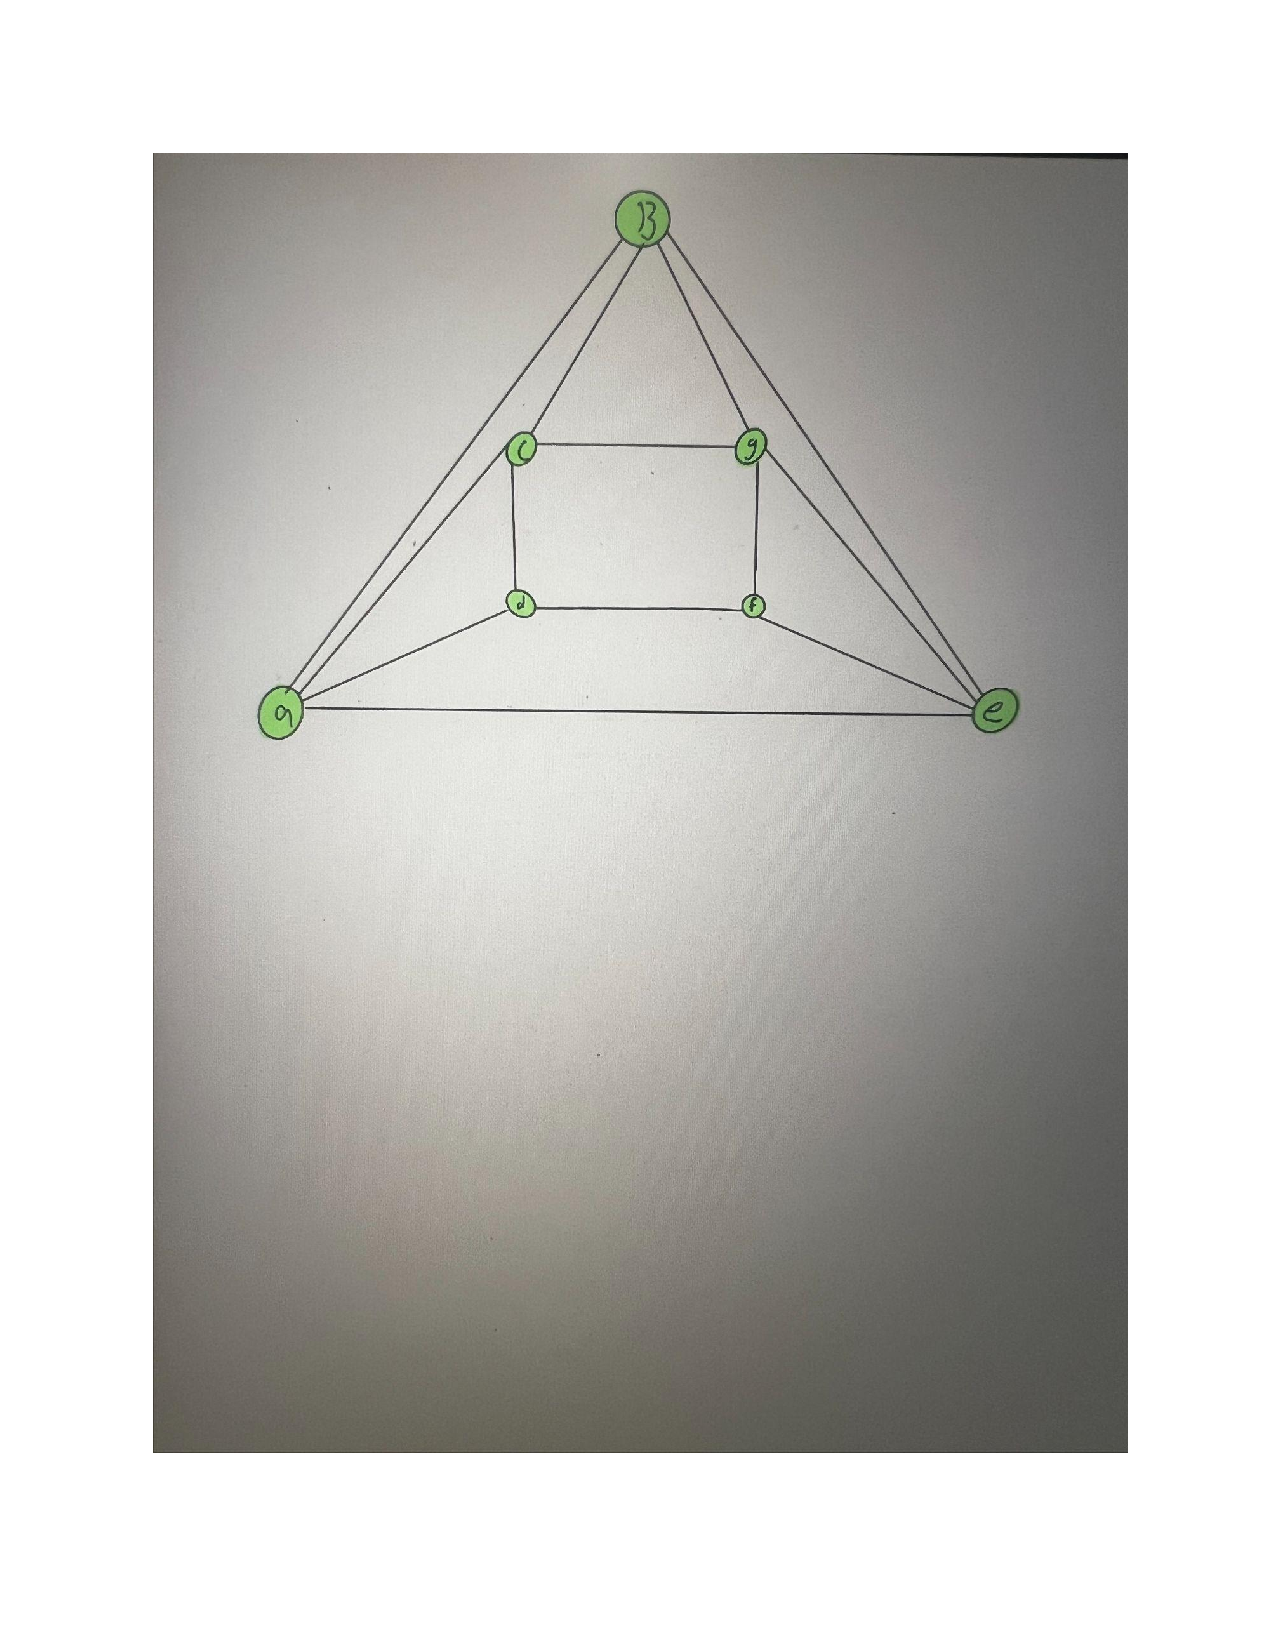
\includegraphics[width=1.75in]{planar_graphG_hw5_solution.pdf}
\end{minipage}
\hfill
{\large Graph $H$:\ }
\begin{minipage}{2.4in}
		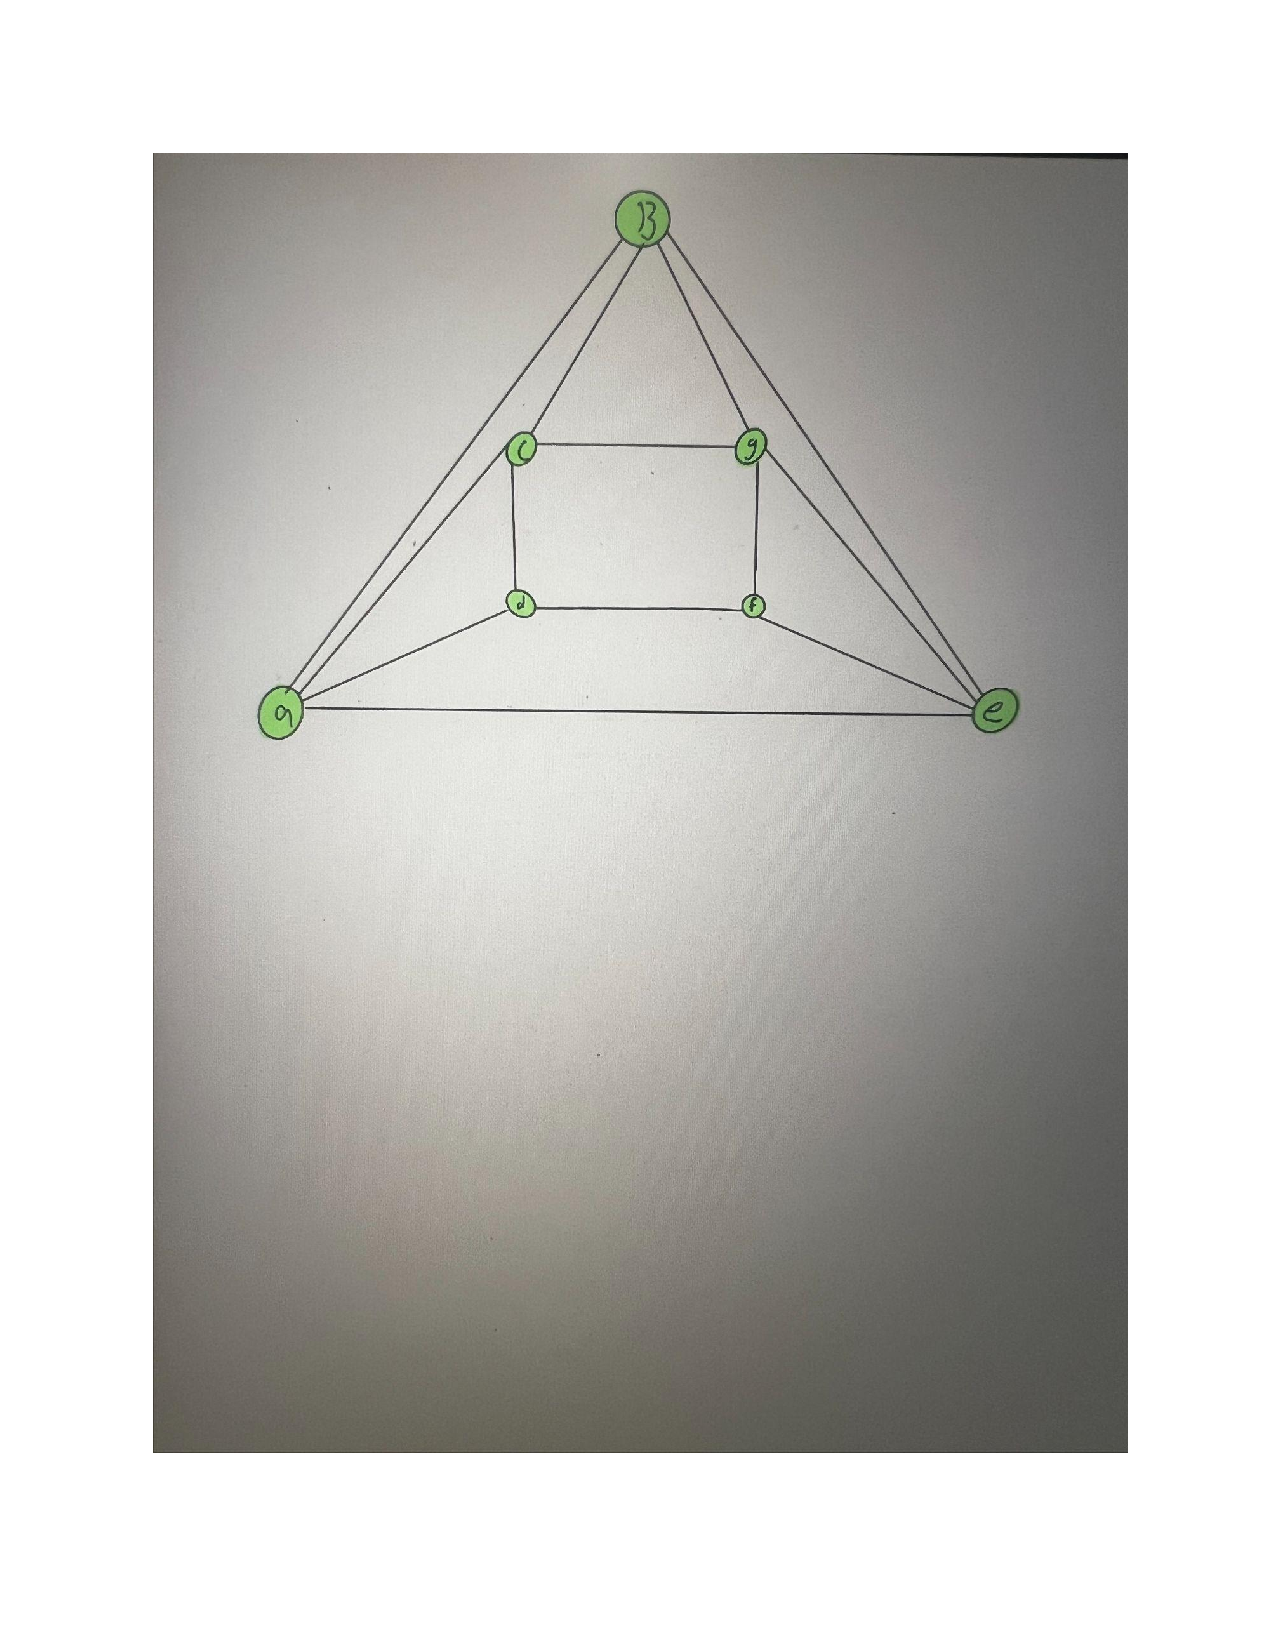
\includegraphics[width=2in]{planar_graphH_hw5_solution.pdf}
\end{minipage}
\end{center}

\vspace{0.1in} - Graph $G$ is planar. The planar embedding is shown above.

\vspace{0.1in} - Graph $H$ is not planar. It contains a subgraph that is a subdivision of $K_{5}$, which is a non-planar graph. Therefore, by Kuratowski's theorem, $H$ is not planar.
\end{problem}

\vskip 0.25in

%%%%%%%%%%%%%%%%%%%%%%%%%%%%

\begin{problem}
	You are given two bipartite graphs $G$ and $H$ below. For each
	graph determine whether it has a perfect matching.
	Justify your answer, either by 
	listing the edges that are in the matching or using
	Hall's Theorem to show that the graph does not have a
	perfect matching.

\vskip 0.25in

	\begin{center}
	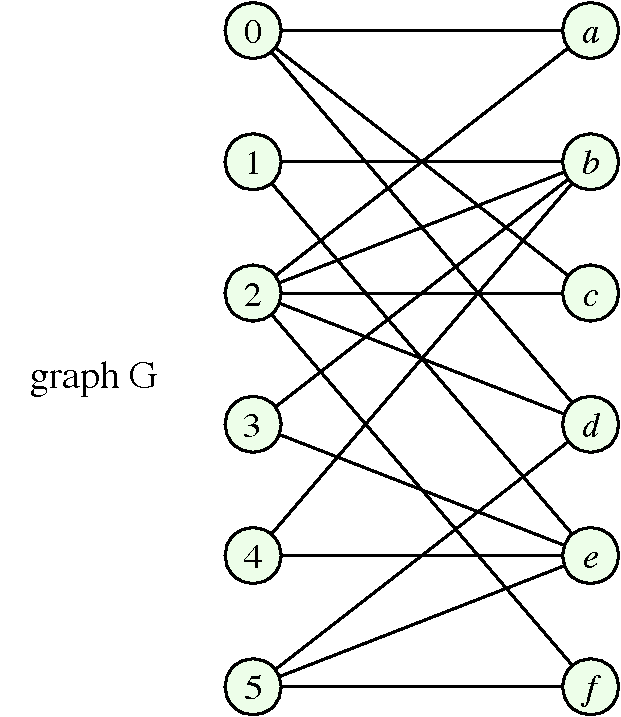
\includegraphics[width = 2.5in]{bipartite_graphG_hw5.pdf}
	\quad\quad
	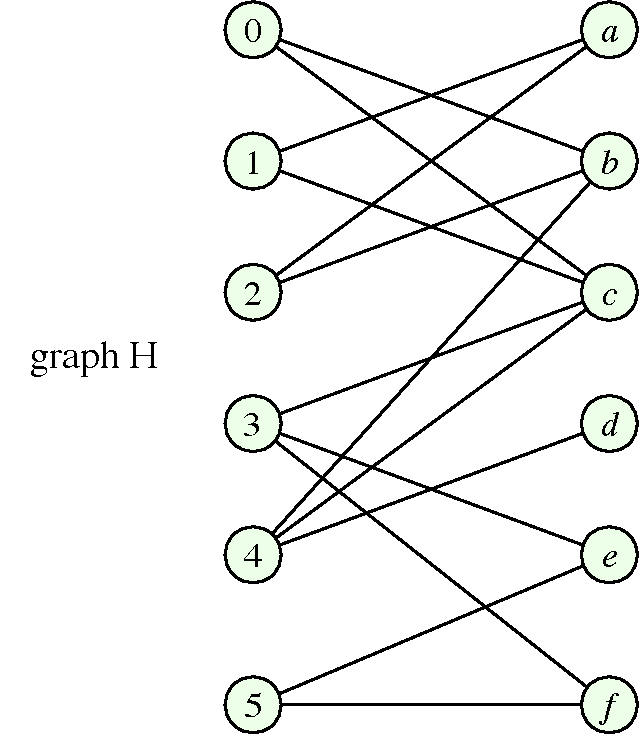
\includegraphics[width = 2.5in]{bipartite_graphH_hw5.pdf}
	\quad\quad\ 
	\hfill\ 
	\end{center}

\vskip 0.25in

\vspace{0.1in} - Graph $G$ does not have a perfect matching. By Hall's Theorem, there is no perfect matching in $H$ because the number of neighbors of $X$ is less than $|X|$ for the set $X = \{a, b, c, d,e,f\}$.

\vspace{0.1in} - Graph $H$ has a perfect matching. The perfect matching is $\{(c,0), (a, 1), (b, 2), (e, 3), (d, 4), (f,5)\}$.

\end{problem}

\vfill
\eject

%%%%%%%%%%%%%%%%%%%%%%%%%%%%

\vskip 0.25in

\begin{problem}
(a) For each degree sequence below, determine whether there is a graph with $6$ vertices where vertices have
these degrees. If a graph exists,  (i) draw it, (ii) find the chromatic number and justify, (iii) determine whether the graph has an Euler tour and justify, (iv) determine whether the graph has a Hamiltonian cycle and justify. If no such graph exists, justify.
%
\begin{description}\setlength{\itemsep}{-3pt}
	\item{(a1)} $5, 5, 4, 4, 3, 1$.  
	\item{(a2)} $5, 5, 4, 3, 3, 1$. 
	\item{(a3)} $5, 5, 5, 4, 4, 3$.
\end{description}

(b) For each degree sequence below, determine whether there is a planar graph with $6$ vertices where vertices have
these degrees. If a planar graph exists, (i) draw it, (ii) find the chromatic number and justify, (iii) determine whether the graph has an Euler tour and justify, (iv) determine whether the graph has a Hamiltonian cycle and justify. If no such planar graph exists, justify.
%
\begin{description}\setlength{\itemsep}{-3pt}
	\item{(b1)} $5, 5, 3, 3, 2, 2$.
	\item{(b2)} $5, 5, 4, 4, 4, 4$.
\end{description}
\end{problem}

%%%%%%%%%%%%%%%%%%%%%%%%%%%%

\paragraph{Academic integrity declaration.}
The homework papers must include at the end an academic integrity declaration. This should be a short paragraph where you briefly explain 
\emph{in your own words}  (1) whether you did the homework individually or in collaboration with a partner student (if so, provide the name), 
and (2) whether you used any external help or resources. 

\vspace{0.1in} - For all the problems above, I referenced all the examples shown in the planar and bipartite graph lecture notes and slides. I 
also used 2 youtube videos to better understand the concepts of planar graphs and bipartite graphs. I did this homework individually.

%%%%%%%%%%%%%%%%%%%%%%%%%%%%

\vskip 0.1in
\paragraph{Submission.}
To submit the homework, you need to upload the pdf file to Gradescope. If you submit with a partner, you need
to put two names on the assignment and submit it as a group assignment.
Remember that only {\LaTeX} papers are accepted. 

\end{document}

